\AtBeginSection[]
{
  \begin{frame}<beamer>
    \frametitle{Exmples \thesection}
    \tableofcontents[currentsection]
  \end{frame}
}

\begin{frame}
  \frametitle{COPERNICUS C3S}

 	\includegraphics[width=1\textwidth]{images/NL_150_-_News_11_-_Fig_1.png}
 %   \caption{Copernicus Climate Change Service (C3S) operated by ECMWF}

\href{https://climate.copernicus.eu/about-c3s}{Copernicus Climate Change Service}

\end{frame}

\begin{frame}
  \frametitle{PAVICS: \\ A Platform for the Analysis and Visualization of Climate Science}

  \begin{tikzpicture}[remember picture,overlay]
      \node[xshift=-6.3cm,yshift=-5.4cm] at (current page.north east)
      {\includegraphics[width=1.1\textwidth]{images/pavics}};
  \end{tikzpicture}

  
% \begin{textblock*}{7cm}(5cm,3cm)
%  \begin{itemize}
%    \item Project based on Birdhouse by Ouranos and CRIM, Canada
%    \item Ouranos needs a platform for climate services
%    \item Creating and delivering climate products
%    \item Make climate research less painful
%  \end{itemize}
% \end{textblock*}

  \vspace{6cm}
  \centering
  \footnotesize{\url{https://www.researchgate.net/project/PAVICS}}
\end{frame}


\begin{frame}
  \frametitle{CODE-DE} 
	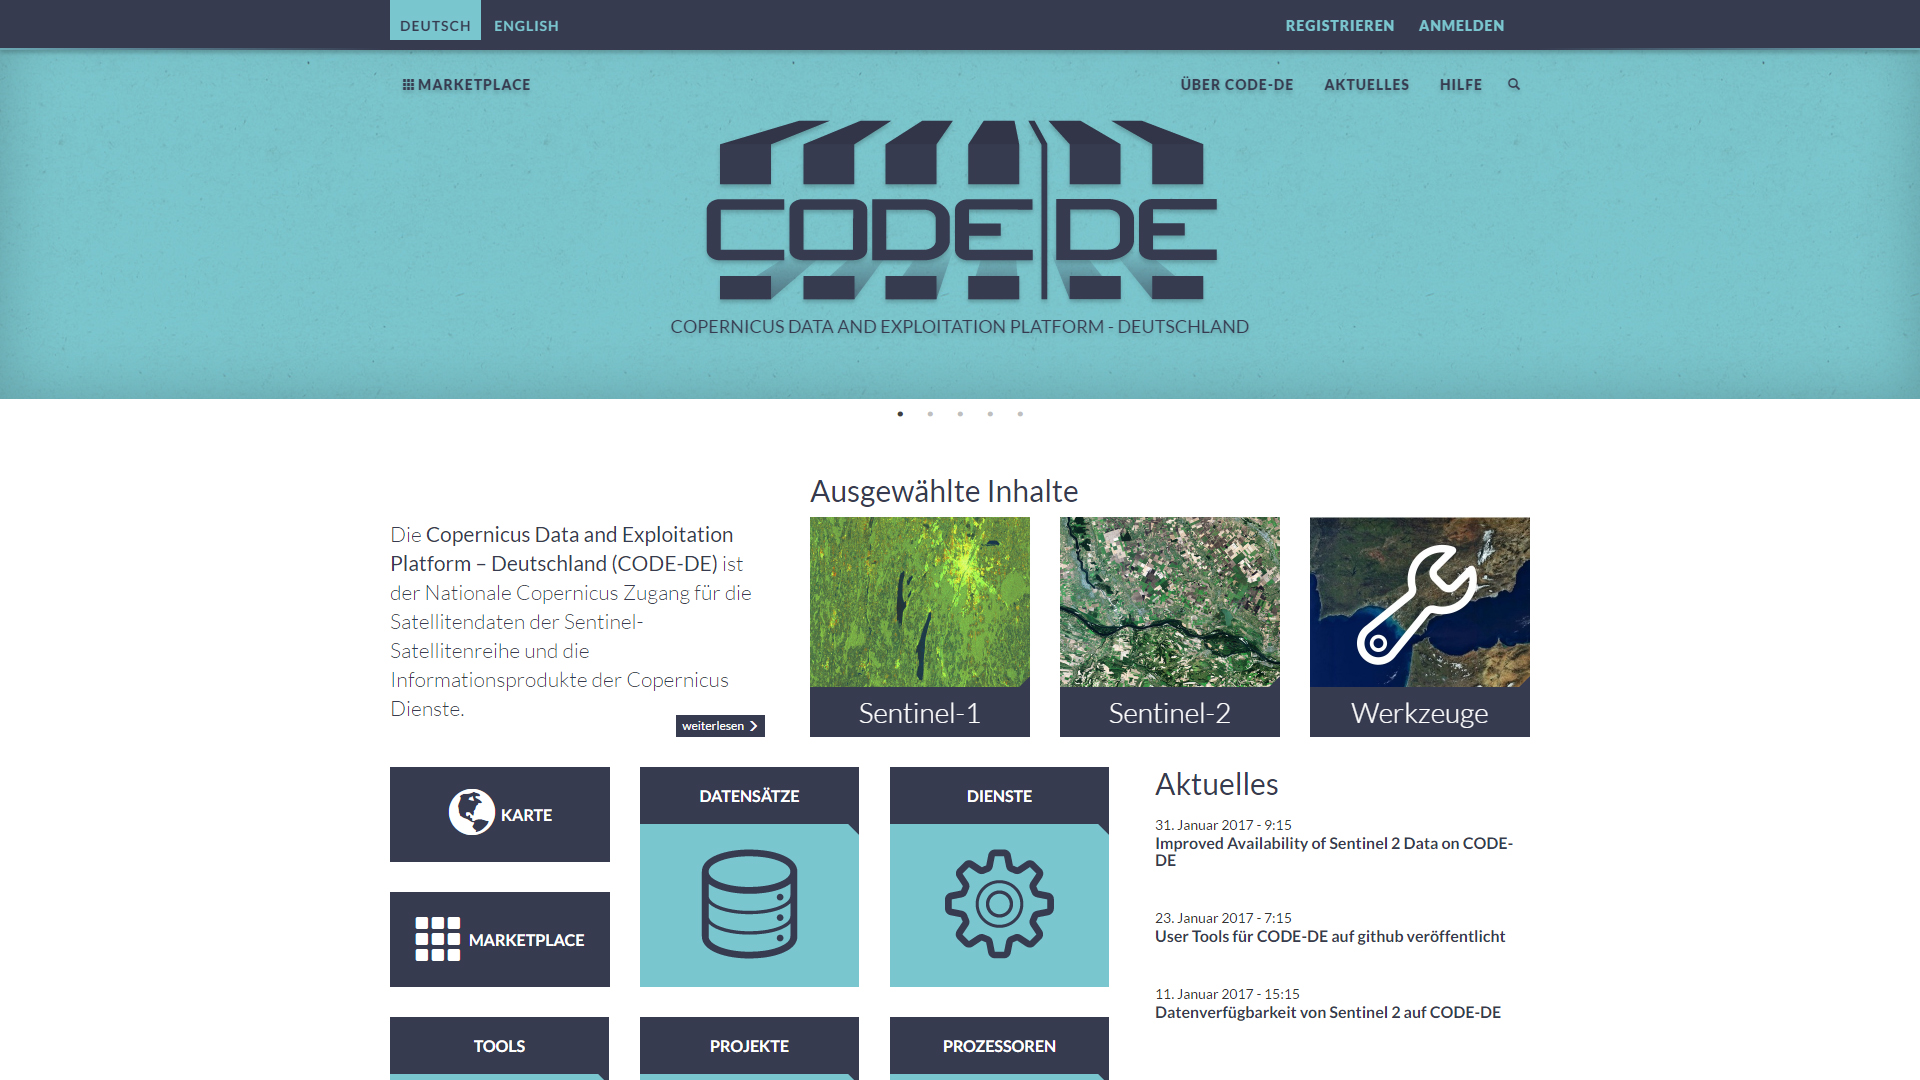
\includegraphics[width=1\textwidth]{images/cde_screen_0001_portal.jpg}\\
    
\href{https://code-de.org/}{code-de.org}
\end{frame}


\begin{frame}
  \frametitle{ TEP ESA }
 \includegraphics[width=1\textwidth]{images/esa_tep.jpg}\\
  
\href{https://tep.eo.esa.int/}{ESA Thematic Exploitation Platforms (TEPs)} 
 
\end{frame}

\begin{frame}
  \frametitle{REDD+ cloud computing tool}

\begin{tikzpicture} %[spy using overlays]
\node (pic1) [inner sep=0pt] {\includegraphics[width=0.3\textwidth,keepaspectratio=true]{./images/sepal_satpics}};

\node (pic2) [inner sep=0pt, anchor=west, yshift=1.5cm, xshift=-.5cm, ] at (pic1.east) {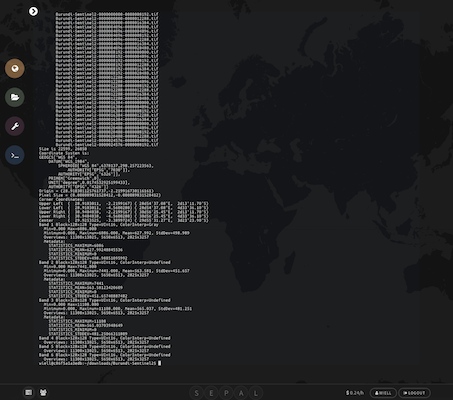
\includegraphics[width=0.3\textwidth]{images/sepal_metadata.png}};
\node (pic3) [inner sep=0pt, anchor=west, yshift=1.5cm, xshift=-.5cm, ] at (pic2.east) {\includegraphics[width=0.3\textwidth]{images/sepal_outout.png}};

\node (link1) [inner sep=0pt, anchor=west, yshift=-2cm, xshift=-.5cm, ] at (pic3.south) {Link: \href{https://sepal.io/}{  sepal.io  } };

\end{tikzpicture}

% node[fill=red!20, ] {3rd node};

\end{frame}

\begin{frame}
  \frametitle{ JICA-JAXA }
 \begin{center}
 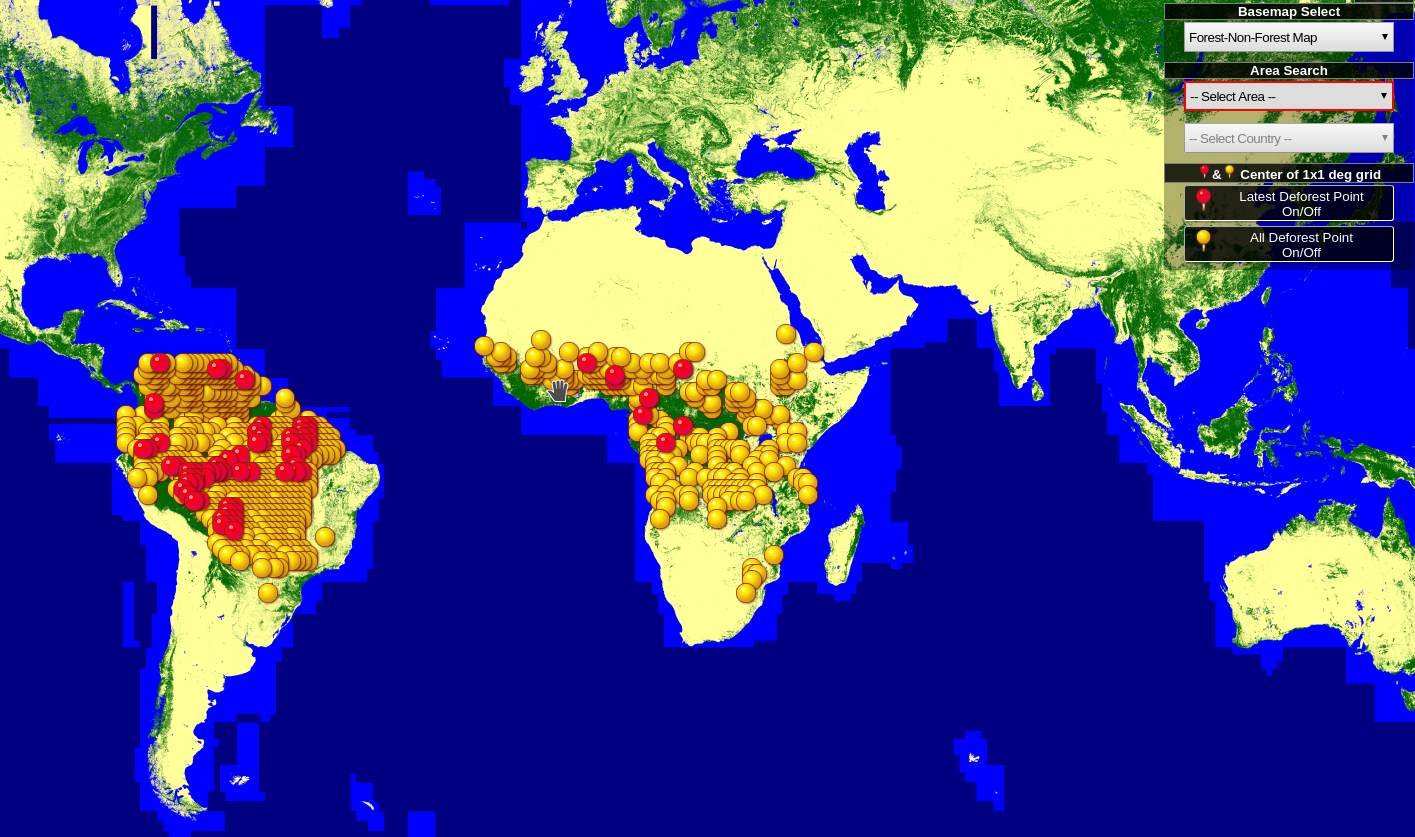
\includegraphics[width=0.9\textwidth,keepaspectratio=true]{./images/jjfast.png}
 % jjfast.png: 0x0 pixel, 300dpi, 0.00x0.00 cm, bb=
\end{center} 

\href{http://www.eorc.jaxa.jp/jjfast/}{JICA-JAXA Forest Early Warning System in the Tropics }
\end{frame}

\begin{frame}
  \frametitle{Trends.earth QGIS plugin (UNCCD LDN --> SDG 13.5.1)} 

\begin{tikzpicture} %[spy using overlays]
\node (pic1) [inner sep=-20pt] {\includegraphics[height=0.25\textheight]{images/trendsearth-0.png}};

\node (pic2) [inner sep=0pt, anchor=west, yshift=1.5cm, xshift=-.5cm, ] at (pic1.east) {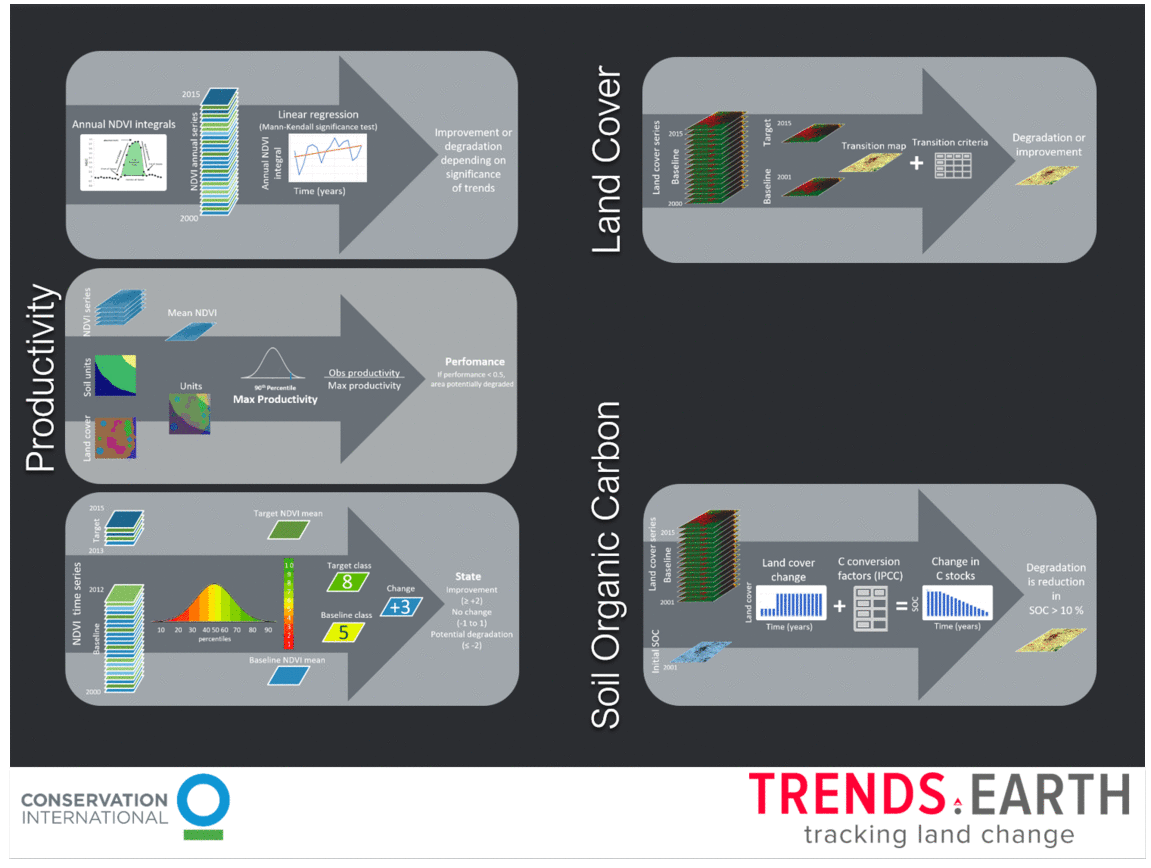
\includegraphics[width=0.3\textwidth]{images/trendsearth-1.png}};


\node (pic3) [inner sep=0pt, anchor=west, yshift=1.5cm, xshift=-1cm, ] at (pic2.east) {\includegraphics[width=0.3\textwidth]{images/trendsearth-2.png}};


\node (pic4) [inner sep=0pt, anchor=north, yshift=-.8cm, xshift=1.5cm, ] at (pic3.south) {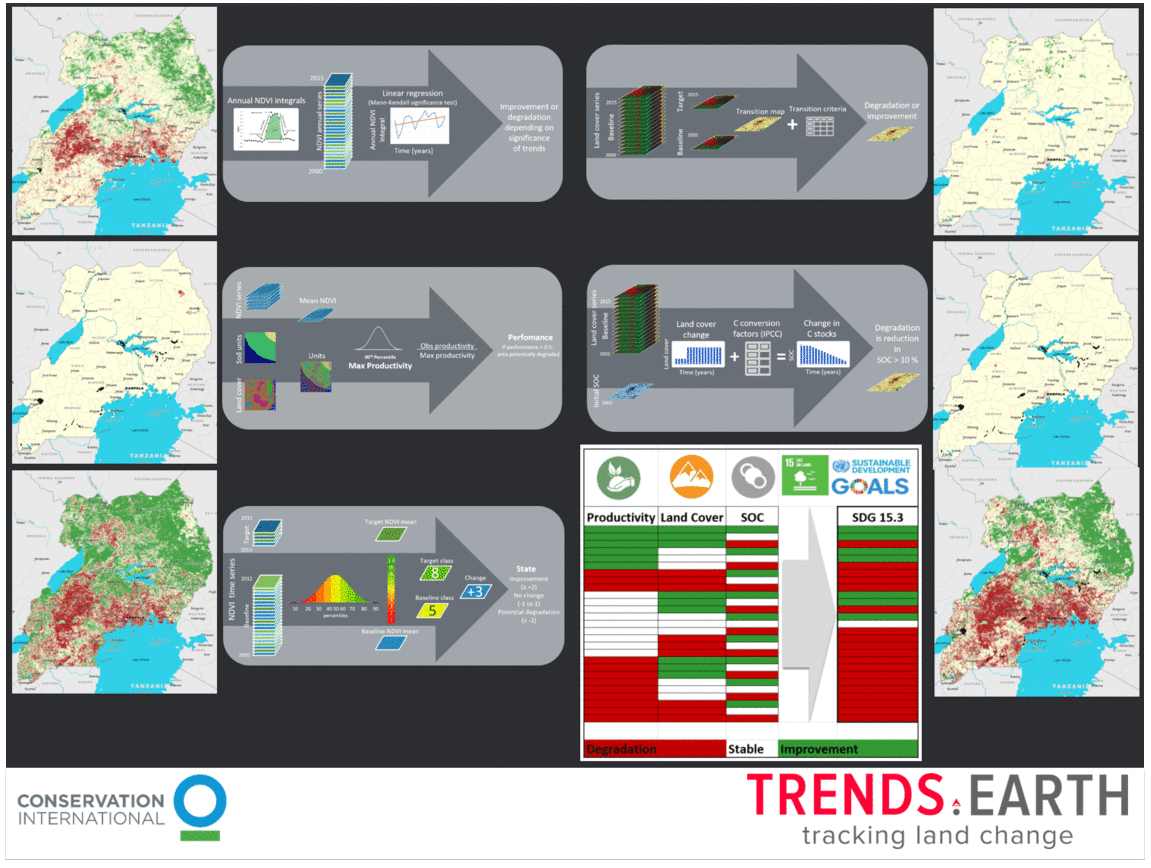
\includegraphics[width=0.3\textwidth]{images/trendsearth-3.png}};


\node (pic5) [inner sep=0pt, anchor=west, yshift=1.5cm, xshift=-1.2cm, ] at (pic4.east) {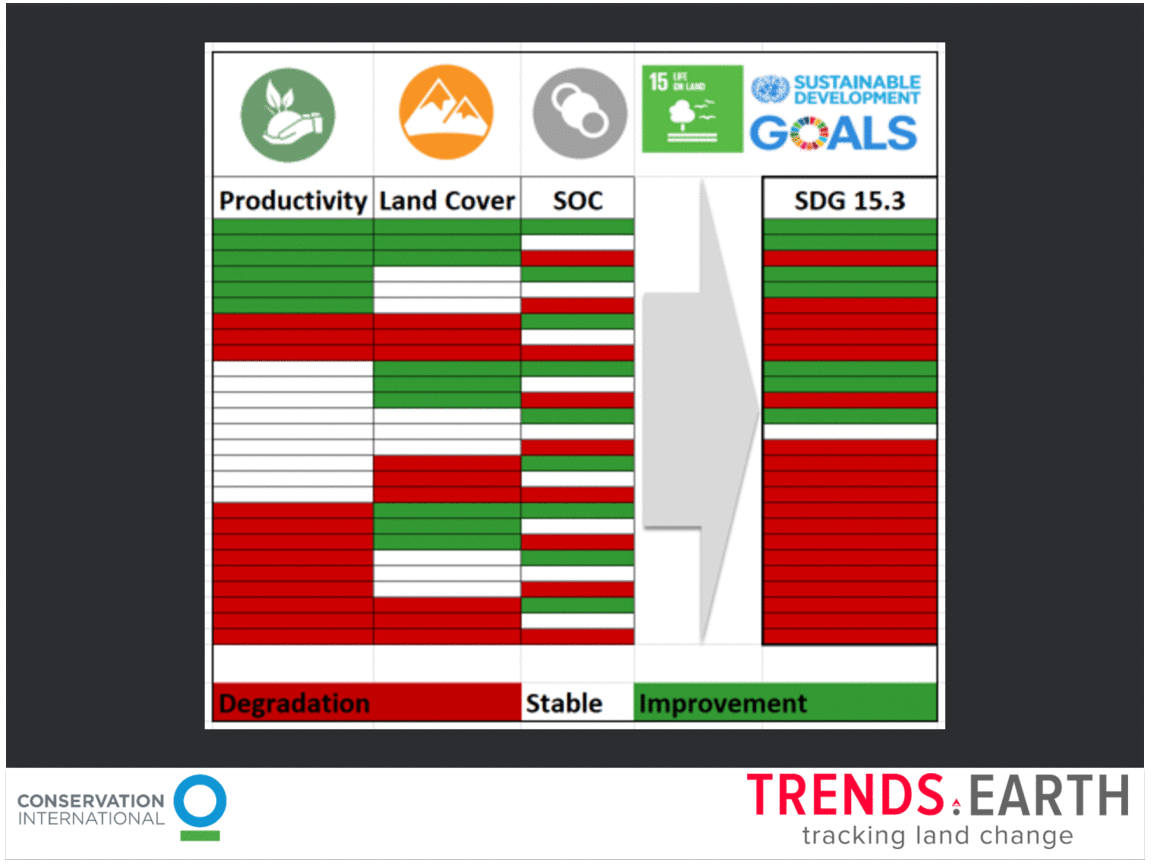
\includegraphics[width=0.3\textwidth]{images/trendsearth-4.png}};


\node (pic6) [inner sep=0pt, anchor=west, yshift=1.7cm, xshift=-1.4cm, ] at (pic5.east) {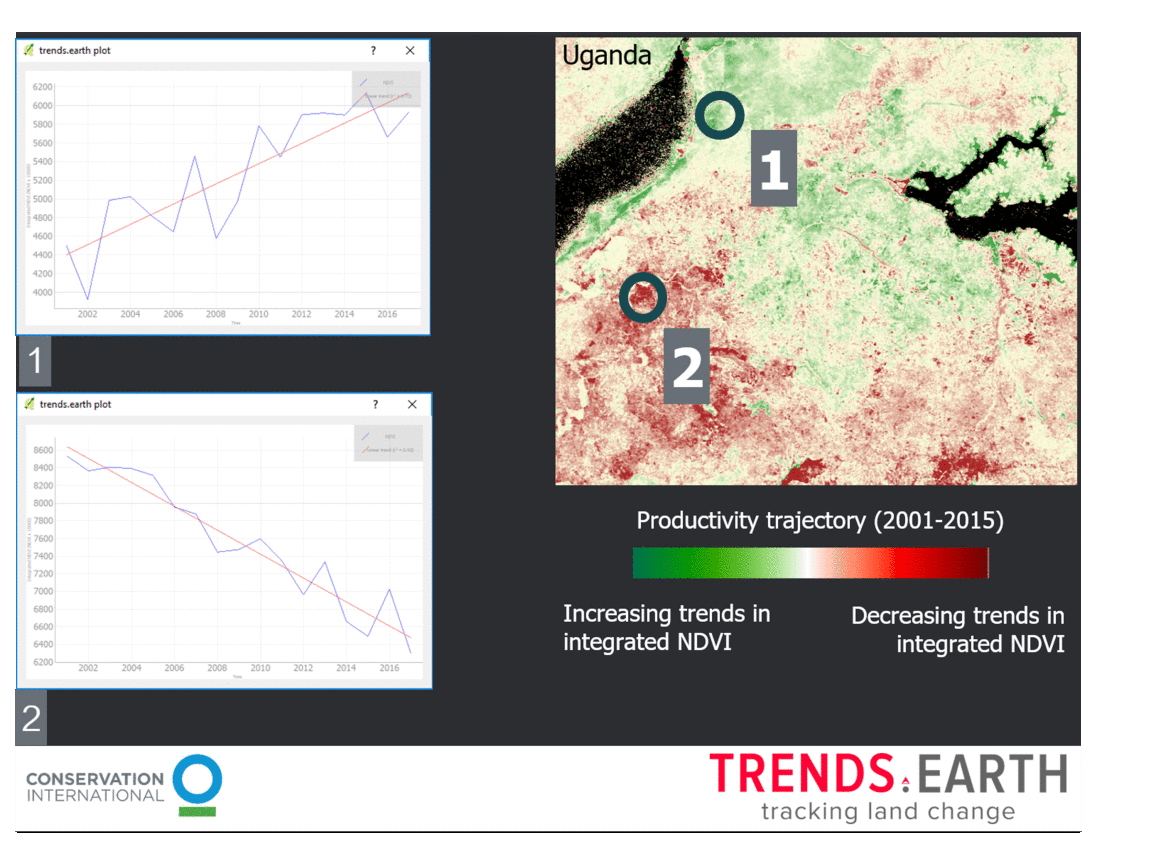
\includegraphics[width=0.3\textwidth]{images/trendsearth-5.png}};
   
   
\end{tikzpicture}

\centering
\href{ http://trends.earth/docs/en/}{link to Documentation Trends.Earth}\\
\href{http://trends.earth/docs/en/documentation/info.html}{link to  Tutorial Trends.Earth}

\end{frame}

\begin{frame}
  \frametitle{ODC}
\vspace{-1.5cm}
\begin{figure}[ht]
	\centering
	\includegraphics[width=0.8\textwidth, page=3]{./images/Sims_SamoaODC_23May2018.pdf}
   % \caption{(Regional Data Cubes \tiny{(Thanks to Neil Sims CEOS)}}
\end{figure}
\href{https://www.opendatacube.org/}{opendatacube}\\
\href{https://www.earthobservations.org/documents/meetings/201805_rapp_sdg_odc/201805_odc_announcement.pdf}{Link: African Regional Data Cube Announcement}\\
\vspace{0.5cm}
Video Links:\\ 
\href{https://www.youtube.com/watch?v=tEeT5VH7qVc}{Africa Regional Data Cube}\\
\href{https://www.youtube.com/watch?v=exIBPwtvbiI}
{How the Data Revolution is Shaping Africa's Future}

\end{frame}

% \begin{frame}
%   \frametitle{ Rangeland and pasture productivity }
%    http://map.geo-rapp.org/
% \end{frame}
